\chapter{Судалгааны үр дүн, дүгнэлт}
\label{ch:results}

\section{Объект таних алгоритмын үр дүн}

Объект таних алгоритмыг YOLOv12 загварт шилжүүлэн сургах аргаар 10,000 зургаас бүрдсэн датасет дээр сургасан бөгөөд, сургалтын үр дүнг статистик хэмжүүрүүдээр үнэлж, симуляцийн орчинд туршин баталгаажуулсан болно.

\subsection{Статистик үр дүн}

Сургалтын үр дүнг үнэлэхэд объект таних чиглэлд өргөн хэрэглэгддэг дараах 4 хэмжүүрийг ашигласан. Эдгээр хэмжүүрүүдэд \textit{(B)} тэмдэглэгээ нь хязгаарлах тэгш өнцөгт \textit{(bounding box)} дээр тооцсоныг илэрхийлнэ.

\begin{itemize}
    \item \textbf{Precision(B)} --- Загварын таамагласан бүх объектуудаас зөв таамагласан объектуудын эзлэх хувь. Өөрөөр хэлбэл, загвар объект гэж зааж байгаа бүрийн хэр нь үнэндээ объект болохыг хэмждэг. Утга нь 1-д ойртох тусам буруу таамаглал \textit{(false positive)} бага байна.
    \item \textbf{Recall(B)} --- Зурган дахь бодит объектуудаас загварын зөв илрүүлсэн объектуудын эзлэх хувь. Өөрөөр хэлбэл, байгаа объектуудыг хэр бүрэн илрүүлж чадаж байгааг хэмждэг. Утга нь 1-д ойртох тусам алдагдсан илрүүлэлт \textit{(false negative)} бага байна.
    \item \textbf{mAP50(B)} --- Таамагласан хязгаарлах тэгш өнцөгт нь зөв хязгаарлах тэгш өнцөгттэй 50\%-иас дээш огтлолцсон тохиолдлуудын бүх ангиллын дундаж нарийвчлал \textit{(mean Average Precision)}.
    \item \textbf{mAP50-95(B)} --- Огтлолцлын босгыг 50\%-аас 95\% хүртэл 5\%-ийн алхамаар өөрчилж тооцсон дундаж нарийвчлал. mAP50-тай харьцуулахад илүү чанд шалгуур бөгөөд, загварын хязгаарлах тэгш өнцөгтийн нарийвчлалыг илэрхийлдэг.
\end{itemize}

Зураг~\ref{fig:training-results}-д үзүүлснээр сургалтын явцад бүх хэмжүүрүүд тогтвортой нэмэгдэж, 100 эпохын дотор тогтворжсон байна. Сургалтын эцсийн үзүүлэлтүүд дараах байдалтай байсан: recall(B) хэмжүүр \textbf{91\%}-д хүрч хамгийн өндөр үзүүлэлт болсон бөгөөд, энэ нь туршилтын датасет дахь бодит объектуудын 91\%-ийг загвар зөв илрүүлж чадсаныг харуулж байна.

\begin{figure}[H]
    \centering
    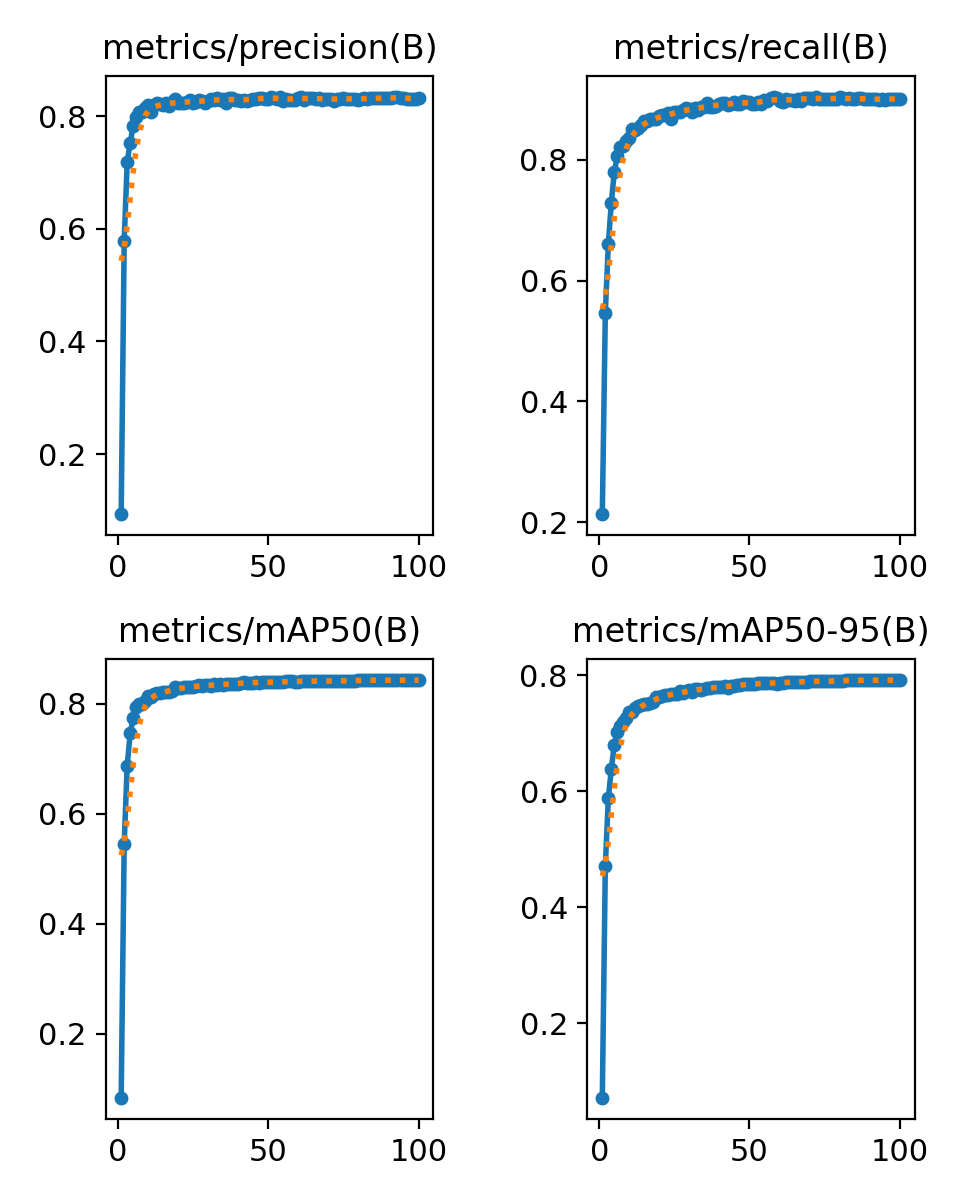
\includegraphics[width=0.5\textwidth]{Pictures/training-results.png}
    \caption{Сургалтын хэмжилтийн үр дүн}
    \label{fig:training-results}
\end{figure}

\subsection{Симуляцийн орчинд туршсан үр дүн}

Сургасан загварыг симуляцийн орчинд HTTP серверээр дамжуулан бодит цагийн горимд \textit{(real-time)} туршилт хийсэн болно. Симуляцийн орчны камерт байнгын дүрс дамжуулж, загварын илрүүлэлтийн үр дүнг шууд харуулсан байна.

\begin{figure}[H]
    \centering
    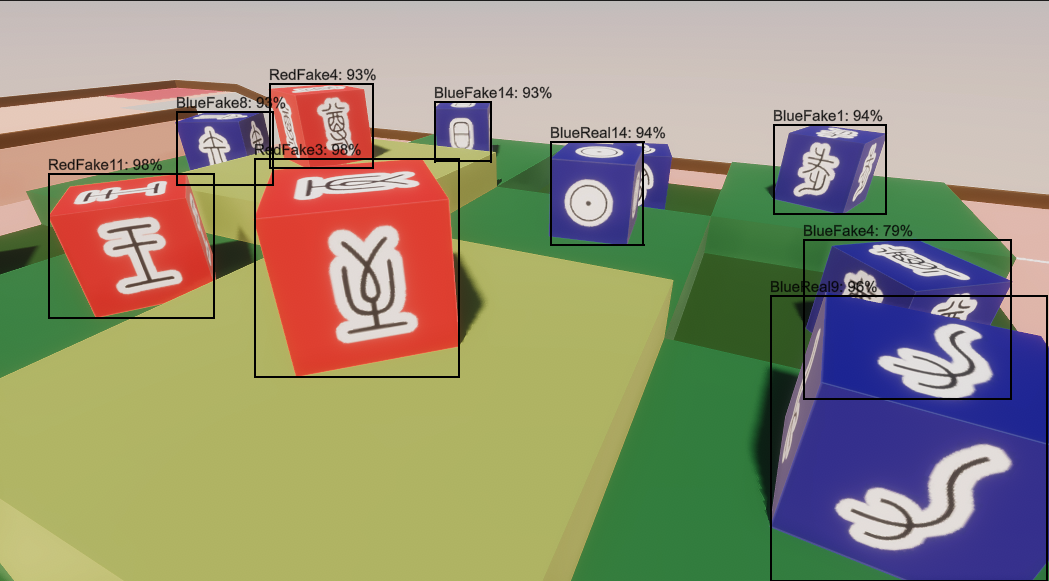
\includegraphics[width=0.9\textwidth]{Pictures/prediction_test.png}
    \caption{Объект таних алгоритмын симуляцийн орчинд хийсэн туршилт}
    \label{fig:simulation-test}
\end{figure}

Зураг~\ref{fig:simulation-test}-д үзүүлснээр танисан объект бүрийн нэршил болон итгэлийн хувийг хязгаарлах тэгш өнцөгтийн хамт харуулсан байна. Туршилтын үр дүнгээс дараах дүгнэлтүүдийг гаргасан:

\begin{enumerate}
    \item \textbf{Өндөр итгэлт илрүүлэлт} --- Ихэнх тохиолдолд объектуудыг \textbf{90\%}-иас дээш итгэлтэйгээр илрүүлсэн байна.
    \item \textbf{Далдлагдсан объектын илрүүлэлт} --- Бусад объектоор хэсэгчлэн далдлагдсан судрыг \textbf{79\%}-ийн итгэлтэйгээр илрүүлж чадсан байна. Энэ нь датасетэд далдлагдсан объектуудын нөхцлийг хангалттай хамарсантай холбоотой.
    \item \textbf{Буруу илрүүлэлтгүй} --- Сургасан ангиллуудаас бусад объектыг объект гэж буруу илрүүлсэн тохиолдол \textit{(false positive)} туршилтын явцад огт ажиглагдаагүй байна.
\end{enumerate}

Сургасан загвар нь нийт 30 ангилалтай байсан бөгөөд, эдгээр нь Зураг~\ref{fig:scroll-classes}-д үзүүлснээр жинхэнэ \textit{(Real)} болон хуурамч \textit{(Fake)} гэсэн 2 бүлэгт хуваагдах 15 төрлийн Күнг-Фү судрыг хамарсан байна.

\begin{figure}[H]
    \centering
    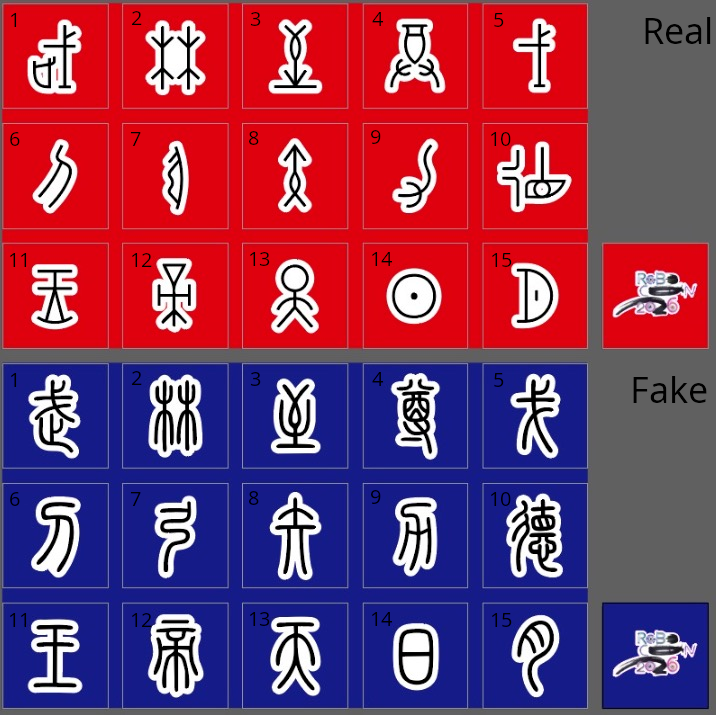
\includegraphics[width=0.8\textwidth]{Pictures/class_indices.png}
    \caption{Күнг-Фү сударын ангилал болон индекс}
    \label{fig:scroll-classes}
\end{figure}
